\documentclass[10pt,twocolumn]{article}
\usepackage[a4paper,margin=15mm]{geometry}
\usepackage{amsmath,amssymb}
\usepackage{amsthm}
\usepackage{graphicx}
\theoremstyle{definition}
\newtheorem{remark}{Remark}
\usepackage{booktabs,array,calc}
\usepackage[font=small,labelfont=bf]{caption}
\usepackage[colorlinks=true]{hyperref}
\providecommand{\tightlist}{\setlength{\itemsep}{0pt}\setlength{\parskip}{0pt}}
\renewcommand{\thesubsection}{\arabic{subsection}.}
\emergencystretch=3em
\allowdisplaybreaks
\setlength{\tabcolsep}{4pt}

\begin{document}
\title{Exact Audits of Worked Systems for the\\
Obstruction Calculus:\\
Counts, Witnesses, and Monitoring Design Rules}
\author{Amin Abaee\\[0.35em]
{\small Independent Researcher}\\[0.55em]
{\small\href{https://orcid.org/0000-0002-0019-1842}{ORCID: 0000-0002-0019-1842}}\\[0.3em]
{\small\href{mailto:amin\_abaee@ut.ac.ir}{amin\_abaee@ut.ac.ir}}}
\date{September 24, 2026}
\maketitle

\begin{abstract}
Viability certificates are useful in application to the extent that their
behaviour on concrete systems is known exactly. This paper develops one
exact audit frame --- integer and rational arithmetic throughout, every
count regenerated by script --- and applies it to a family of worked
systems that instantiate the mechanisms of the obstruction calculus
(Abaee, 2026b): a shared finite two-coordinate system with observation
structures (aggregation, policy-class restrictions, decentralized
observation, regime uncertainty), a review-timing grid for a
hidden-regime resource model, and a continuous two-floor production
benchmark. The audits yield the following. The review-timing identity on
the 48-cell grid is non-strict: viability at the deadline holds if and
only if \(T_{\mathrm{obs}} \le \sigma^{*}(z_0) = z_0 - 1\), boundary
included; the strict form fails at exactly one cell. On the four-state
monitoring target, 7 of the 15 partitions are adequate with two minimal
two-cell partitions, and the two maximal common-action sets overlap, so
no coarsest adequate design exists. Four policy classes have kernel
sizes 24, 26, 25, and 28 of 36 belief pairs, forming a Boolean product
with incomparable middle cells. Decentralized unanimity over a
\(256\)-law space sustains 12 of 36 pairs; an authority restriction
collapses the kernel to zero. Mode-blind operation loses exactly the
pairs containing one state. The biased certainty-equivalence law has
drift at least \(21/100\) on \([1,2]\); the bias-free law has drift
identically zero. The benchmark's critical aggregate is \(Y^{*} = 27/5\),
with a rational dual certificate of margin \(3/50\). Static duality
holds at value \(-1/10\) on the two-floor instance with a normalized
Farkas pair, and a Helly-tight triple exhibits the sparse \(m{+}1\)-point
witness. The complete result tables are carried here: the master table
of all 36 belief pairs against the five kernels, the sixteen sustaining
law pairs of the decentralized protocol (an exact \(4 \times 4\)
product), the 48-cell timing grid, the fifteen-partition census with
each fibre's common safe-action set, and the benchmark and drift tables,
with a five-figure set regenerated from the same scripts. Design rules
follow: review deadlines are boundary-inclusive; merged fibres call for
splits, not threshold tuning; aggregated indices support certainly-safe
reporting only; biased observation maps call for structural correction.
\end{abstract}

\textbf{Keywords:} viability kernels; obstruction certificates; exact
arithmetic; monitoring design; decentralized observation; certainty
equivalence

\subsection{Introduction}\label{introduction}

The obstruction calculus states sound sufficient conditions for
nonviability --- obstruction certificates --- mechanism by mechanism:
common-action failure, review-timing failure, tube failure, finite-time
exit, certification failure through fibre crossing, and failure induced
by restricting the policy class (Abaee, 2026b). Each mechanism is
accompanied in application by quantitative questions. How many belief
states does an observation structure destroy, and which ones? At which
review deadlines does the timing certificate fire, and does it fire at
the boundary? What exactly does a vote protocol cost, and which law in
the protocol's space sustains a given target? This paper answers such
questions exactly for a family of worked systems, under one audit frame
and one notation.

Three properties define the frame. First, all computations are carried
out in integer and rational arithmetic: no solver, no tolerance, no
simulation. Second, every system in the family is finite and every count
is regenerated by a deterministic standard-library script, so any two
executions agree. Third, each audited quantity is stated together with a
witness or a certificate --- an action sequence, a partition, a law
pair, a dual measure --- so the counts carry their own evidence. This
edition carries the audit's complete result tables and its figure set:
the per-pair membership table behind the kernel counts, the sustaining
law pairs behind the decentralized count, the full timing grid, the full
partition census, and the benchmark and drift tables, every entry of
which is regenerated from the same scripts that verify the text.

The systems are drawn from the applied model of Abaee (2026a), in which
a two-coordinate resource stock is managed by acting one of two
instruments under incomplete observation. The family comprises: the
shared audit system with its observation structures (Sections
\ref{master}--\ref{regimes}); the hidden-regime review grid (Section
\ref{timing}); a continuous two-floor production benchmark (Section
\ref{benchmark}); and a multiple-floor line extending the Farkas
certificate to jointly binding constraints (Section \ref{floors}).

\subsection{Systems, conventions, and methods}\label{frame}

\emph{The shared audit system.} States are pairs
\(x = (z_1, z_2) \in \{0,1,2,3\}^{2}\); the safe set is
\(\mathcal{V} = \{z_1 \ge 1,\ z_2 \ge 1\}\) with the two coordinates as
floors. Instruments are \(u \in \{0, 1, 2\}\): \(u = j \in \{1,2\}\)
acts coordinate \(j\), which regenerates one unit up to the cap \(3\),
while the other coordinate loses one unit; \(u = 0\) executes no
instrument and both coordinates lose one. The corner \((1,1)\) is the
single state from which no instrument maintains both floors, so its
singleton is nonviable; the nine viable states generate
\(C(9,2) = 36\) two-element belief pairs, the audited population, at
review horizon \(H = 12\) under the audited two-horizon verdict (the
winning recursion at \(H\) and at \(H - 2\); Abaee, 2026b, Theorem 1).

\emph{Observation structures.} An observation map
\(\mathrm{info}: x \mapsto c\) partitions a belief into fibres; a policy
acts per fibre on the read cell. The audited policy classes combine two
aggregation levels (full information; aggregation
\(c(x) = z_1 + z_2\)) with two protocols (free per-step choice; the
no-repeat protocol that forbids repeating the previous action).

\emph{Exactness.} Counts are computed by backward recursion over fibre
partitions with exact state arithmetic; witnesses are extracted as
step-one per-fibre action vectors along a winning branch. The census of
Section \ref{adequacy} enumerates all \(15\) partitions of a four-state
target. The continuous objects of Section \ref{benchmark} are rationals.

\emph{Conventions.} On the hold class of the hidden-regime model, the
discrete survival supremum is \(\sigma^{*}(z_0) = \lfloor z_0 - 1
\rfloor\), with level sets \(\{z_0 \ge 1 + k\}\). Two
certainty-equivalence laws are audited: an uncorrected law whose index
leads the state by one step, \(s \mapsto s + 0.1\), and a corrected law
with the lead removed; both are read through the index \(g(s) = s^{2}\).

\emph{Figures and tables.} Every figure and every tabulated entry in
this paper is produced by a generation script that first recomputes the
quantity from the primitives above, in exact rational arithmetic, and
asserts it before drawing or printing; the master verification script of
Section \ref{methods} chains both scripts and re-derives the tabulated
entries independently.

\subsection{The master table}\label{master}

Table \ref{tab:master} is the audit's master table: all 36 belief pairs
against the five kernels --- the four policy classes of Section
\ref{classes} (institutional, aggregate, full-information codex,
full-information) and the decentralized kernel of Section
\ref{decentralized}. Rows are grouped by the pair's lexicographically
smaller state, written \(z_1 z_2\).

\begin{table*}[t]
\centering
\footnotesize
\caption{The master table: membership of all 36 belief pairs in the five
audited kernels. I = institutional (aggregation, no-repeat); A =
aggregate; C = full-information codex; F = full information; D =
decentralized unanimity. A dot marks a non-member; every entry is
regenerated by script.}
\label{tab:master}
\begin{tabular}{@{}l cccc c@{\hspace{12pt}}l cccc c@{}}
\toprule
Pair & I & A & C & F & D & Pair & I & A & C & F & D\\
\midrule
$12|21$ & $\cdot$ & $\cdot$ & $\cdot$ & F & D &
$22|31$ & I & A & C & F & D\\
$12|31$ & $\cdot$ & A & $\cdot$ & F & $\cdot$ &
$22|23$ & I & A & C & F & $\cdot$\\
$12|23$ & I & A & C & F & D &
$22|33$ & I & A & C & F & D\\
$12|33$ & I & A & C & F & $\cdot$ &
$22|32$ & I & A & C & F & $\cdot$\\
$12|22$ & I & A & C & F & $\cdot$ &
$23|31$ & I & A & C & F & $\cdot$\\
$12|32$ & I & A & C & F & D &
$23|33$ & I & A & C & F & $\cdot$\\
$12|13$ & I & A & C & F & $\cdot$ &
$23|32$ & I & A & C & F & D\\
$13|21$ & $\cdot$ & A & $\cdot$ & F & $\cdot$ &
$31|33$ & I & A & C & F & D\\
$13|31$ & $\cdot$ & $\cdot$ & C & F & D &
$31|32$ & I & A & C & F & $\cdot$\\
$13|23$ & I & A & C & F & $\cdot$ &
$32|33$ & I & A & C & F & $\cdot$\\
$13|33$ & I & A & C & F & D &
$11|12$ & $\cdot$ & $\cdot$ & $\cdot$ & $\cdot$ & $\cdot$\\
$13|22$ & I & A & C & F & D &
$11|21$ & $\cdot$ & $\cdot$ & $\cdot$ & $\cdot$ & $\cdot$\\
$13|32$ & I & A & C & F & $\cdot$ &
$11|31$ & $\cdot$ & $\cdot$ & $\cdot$ & $\cdot$ & $\cdot$\\
$21|31$ & I & A & C & F & $\cdot$ &
$11|23$ & $\cdot$ & $\cdot$ & $\cdot$ & $\cdot$ & $\cdot$\\
$21|23$ & I & A & C & F & D &
$11|33$ & $\cdot$ & $\cdot$ & $\cdot$ & $\cdot$ & $\cdot$\\
$21|33$ & I & A & C & F & $\cdot$ &
$11|22$ & $\cdot$ & $\cdot$ & $\cdot$ & $\cdot$ & $\cdot$\\
$21|22$ & I & A & C & F & $\cdot$ &
$11|32$ & $\cdot$ & $\cdot$ & $\cdot$ & $\cdot$ & $\cdot$\\
$21|32$ & I & A & C & F & D &
$11|13$ & $\cdot$ & $\cdot$ & $\cdot$ & $\cdot$ & $\cdot$\\
\bottomrule
\end{tabular}
\end{table*}

The column counts are the audited kernel sizes
\(|\mathcal{W}_{\mathrm{inst}}| = 24\),
\(|\mathcal{W}_{\mathrm{agg}}| = 26\),
\(|\mathcal{W}_{\mathrm{full\text{-}codex}}| = 25\),
\(|\mathcal{W}_{\mathrm{full}}| = 28\), and
\(|\mathcal{W}_{\mathrm{dec}}| = 12\). Figure \ref{fig:kernels} displays
the four policy-class kernels as a Boolean product with incomparable
middle cells. Two set-level facts are recorded exactly. The meet of the
two middle kernels equals the institutional kernel setwise. At class
level the join is the full-information class; at kernel level the union
of the two middle kernels falls one pair short of the full kernel:
exactly the pair \(\{(1,2),(2,1)\}\) lies in neither middle kernel. The
pair is the alternation-forced pair --- each branch survives only under
its own instrument, so the belief wins only by alternating \(1\) and
\(2\) --- which aggregation cannot see (one fibre, no common action) and
the no-repeat protocol forbids. The full kernel is exactly the
\(C(8,2) = 28\) pairs avoiding the corner \((1,1)\): the corner's
singleton nonviability accounts for every remaining pair-level loss at
full information, as the eight \(11|\cdot\) rows of Table
\ref{tab:master} show.

\begin{figure}[t]
\centering
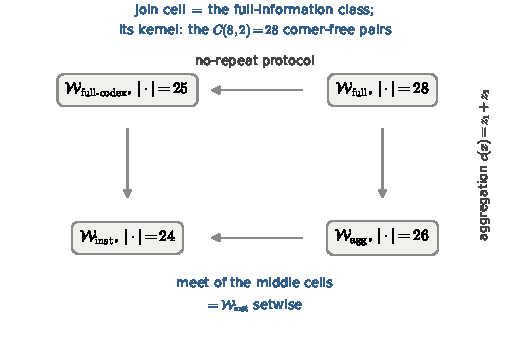
\includegraphics[width=0.94\linewidth]{figs_ws4/fig_kernels.pdf}
\caption{The four policy classes form a Boolean product of aggregation
level and protocol; the audited kernel sizes are \(24, 26, 25, 28\) of
36. The meet of the middle kernels is the institutional kernel setwise;
the class join is the full-information class, whose kernel is the 28
corner-free pairs, one pair beyond the middle-kernel union.}
\label{fig:kernels}
\end{figure}

\subsection{Policy classes}\label{classes}

The four audited classes combine full information and aggregation with
free and no-repeat protocols. Their kernels among the 36 pairs have
sizes:
\begin{gather*}
|\mathcal{W}_{\mathrm{inst}}| = 24,\quad
|\mathcal{W}_{\mathrm{agg}}| = 26,\\
|\mathcal{W}_{\mathrm{full\text{-}codex}}| = 25,\quad
|\mathcal{W}_{\mathrm{full}}| = 28 .
\end{gather*}
The four cells form a Boolean product with incomparable middle cells:
the aggregate kernel contains pairs outside the full-information codex
kernel (for instance \(\{(1,2),(3,1)\}\) and \(\{(1,3),(2,1)\}\)), and
the codex kernel contains pairs outside the aggregate (for instance
\(\{(1,3),(3,1)\}\)). Neither protocol dominance holds. The precise
meet-and-join reading is the one recorded in Section \ref{master}. Two
per-pair readings illustrate the columns of Table \ref{tab:master}. The
pair \(\{(1,2),(3,1)\}\) is aggregate-viable but not codex-viable: the
two branches read distinct fibres under aggregation, so the no-repeat
protocol never binds, while at full information the winning branch
sequence forces a repeated instrument. The pair \(\{(1,3),(3,1)\}\) is
codex-viable but not aggregate-viable: the two branches share the fibre
\(c = 4\), and no single per-fibre instrument serves both, while
full information separates them.

\subsection{Decentralized observation}\label{decentralized}

Two agencies each observe one coordinate and vote; an instrument
executes only on agreement. Each agency's vote is a map from its
coordinate's four values to the two instruments, so the law space has
\(2^{4} \times 2^{4} = 256\) law pairs. Unanimity sustains 12 of the
36 pairs (column D of Table \ref{tab:master}), and exactly 16
coordinated-viable pairs are lost. The loss instance
\(\{(1,2),(3,1)\}\) is representative: each branch is individually
sustainable, and no law pair sustains the belief. For the audited belief
\(\{(1,2),(2,1)\}\), exactly 16 of the 256 law pairs sustain it; the
count coincides numerically with the 16 lost pairs, and no identity is
implied.

\begin{table}[t]
\centering
\footnotesize
\caption{The 16 law pairs sustaining the audited belief
\(\{(1,2),(2,1)\}\) factor exactly: agency 1's vote is forced to
\(1\) at \(z_1 = 1\) and \(2\) at \(z_1 = 2\), free at
\(z_1 \in \{0, 3\}\); agency 2's vote is forced to \(2\) at
\(z_2 = 1\) and \(1\) at \(z_2 = 2\), free at
\(z_2 \in \{0, 3\}\). Every combination sustains --- a complete
\(4 \times 4\) product (votes listed as
\((l(z{=}0), l(z{=}1), l(z{=}2), l(z{=}3))\)).}
\label{tab:laws}
\begin{tabular}{@{}l cccc@{}}
\toprule
 & \multicolumn{4}{c}{agency 2}\\
\cmidrule(l){2-5}
agency 1 & 1211 & 1212 & 2211 & 2212\\
\midrule
1121 & \checkmark & \checkmark & \checkmark & \checkmark\\
1122 & \checkmark & \checkmark & \checkmark & \checkmark\\
2121 & \checkmark & \checkmark & \checkmark & \checkmark\\
2122 & \checkmark & \checkmark & \checkmark & \checkmark\\
\bottomrule
\end{tabular}
\end{table}

The sustaining set has an exact product structure (Table
\ref{tab:laws}): on the trajectory alternating between the branches,
agency 1 is read only at \(z_1 \in \{1, 2\}\) and must vote \(1\) then
\(2\); agency 2 is read only at \(z_2 \in \{2, 1\}\) and must vote
\(1\) then \(2\); the votes at the unreachable coordinates
\(z \in \{0, 3\}\) are free, giving \(2^{2} \times 2^{2} = 16\). Forbidding
agency 2's vote (fixing it to instrument 1) collapses the kernel from
12 to 0: the second agency's voice, not the first's, carries the audited
target. Two modelling choices are declared. The deadlock transition
\(u = 0\) executes no instrument and both coordinates lose one; and
each agency votes on its own coordinate's current value, so the
protocol carries local memory with delay, not common knowledge.

\subsection{Review timing on the hidden-regime grid}\label{timing}

The hidden-regime resource model is audited on the grid
\(z_0 \in \{1.0, 1.1, \dots, 2.5\}\) and
\(T_{\mathrm{obs}} \in \{1, 2, 3\}\), 48 cells. Viability at the
deadline holds if and only if
\(T_{\mathrm{obs}} \le \sigma^{*}(z_0) = z_0 - 1\), with zero
mismatches across the grid. The identity is boundary-inclusive: at the
cell \((z_0, T_{\mathrm{obs}}) = (2, 1)\), on the boundary
\(z_0 = 1 + T_{\mathrm{obs}}\), the system is viable, and the strict
form \(T_{\mathrm{obs}} < \sigma^{*}(z_0)\) fails at exactly this cell.
Table \ref{tab:timing} carries the full grid and Figure
\ref{fig:timing} displays it. The practical form of the rule: a review
must land no later than the worst-case exit time, and a deadline exactly
at the worst-case exit is admissible.

\begin{table}[t]
\centering
\footnotesize
\caption{The 48-cell timing grid: viability at the deadline against
\(\sigma^{*}(z_0) = \lfloor z_0 - 1 \rfloor\). The checkmark of column
\(T_{\mathrm{obs}}\) means the cell is viable; the identity
column ``id.'' is the predicate
\(T_{\mathrm{obs}} \le \sigma^{*}(z_0)\) and column ``cell'' the audited
viability; the two agree on all \(48\) cells (zero mismatches; six
viable cells). The circled cell of Figure \ref{fig:timing} is
\((2.0, 1)\): viable, on the boundary, the only cell where the strict
form disagrees.}
\label{tab:timing}
\begin{tabular}{@{}l c c cc c cc c@{}}
\toprule
 & & \multicolumn{2}{c}{$T_{\mathrm{obs}} = 1$} &
\multicolumn{2}{c}{$T_{\mathrm{obs}} = 2$} &
\multicolumn{2}{c}{$T_{\mathrm{obs}} = 3$}\\
\cmidrule(lr){3-4}\cmidrule(lr){5-6}\cmidrule(lr){7-8}
$z_0$ & $\sigma^{*}$ & id. & cell & id. & cell & id. & cell\\
\midrule
1.0 & 0 & $\cdot$ & $\cdot$ & $\cdot$ & $\cdot$ & $\cdot$ & $\cdot$\\
1.1 & 0 & $\cdot$ & $\cdot$ & $\cdot$ & $\cdot$ & $\cdot$ & $\cdot$\\
1.2 & 0 & $\cdot$ & $\cdot$ & $\cdot$ & $\cdot$ & $\cdot$ & $\cdot$\\
1.3 & 0 & $\cdot$ & $\cdot$ & $\cdot$ & $\cdot$ & $\cdot$ & $\cdot$\\
1.4 & 0 & $\cdot$ & $\cdot$ & $\cdot$ & $\cdot$ & $\cdot$ & $\cdot$\\
1.5 & 0 & $\cdot$ & $\cdot$ & $\cdot$ & $\cdot$ & $\cdot$ & $\cdot$\\
1.6 & 0 & $\cdot$ & $\cdot$ & $\cdot$ & $\cdot$ & $\cdot$ & $\cdot$\\
1.7 & 0 & $\cdot$ & $\cdot$ & $\cdot$ & $\cdot$ & $\cdot$ & $\cdot$\\
1.8 & 0 & $\cdot$ & $\cdot$ & $\cdot$ & $\cdot$ & $\cdot$ & $\cdot$\\
1.9 & 0 & $\cdot$ & $\cdot$ & $\cdot$ & $\cdot$ & $\cdot$ & $\cdot$\\
2.0 & 1 & \checkmark & \checkmark & $\cdot$ & $\cdot$ & $\cdot$ & $\cdot$\\
2.1 & 1 & \checkmark & \checkmark & $\cdot$ & $\cdot$ & $\cdot$ & $\cdot$\\
2.2 & 1 & \checkmark & \checkmark & $\cdot$ & $\cdot$ & $\cdot$ & $\cdot$\\
2.3 & 1 & \checkmark & \checkmark & $\cdot$ & $\cdot$ & $\cdot$ & $\cdot$\\
2.4 & 1 & \checkmark & \checkmark & $\cdot$ & $\cdot$ & $\cdot$ & $\cdot$\\
2.5 & 1 & \checkmark & \checkmark & $\cdot$ & $\cdot$ & $\cdot$ & $\cdot$\\
\bottomrule
\end{tabular}
\end{table}

\begin{figure}[t]
\centering
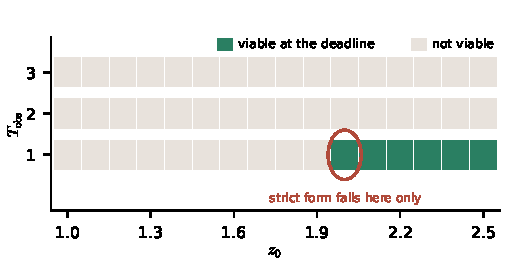
\includegraphics[width=0.96\linewidth]{figs_ws4/fig_timing.pdf}
\caption{The timing grid. Cells viable at the deadline (green) satisfy
\(T_{\mathrm{obs}} \le \sigma^{*}(z_0)\); the identity is
boundary-inclusive, and the strict form fails at exactly one cell,
\((z_0, T_{\mathrm{obs}}) = (2.0, 1)\) (circled).}
\label{fig:timing}
\end{figure}

\subsection{Monitoring adequacy}\label{adequacy}

Let \(R(x)\) denote the safe actions of state \(x\): those keeping
\(x\) in \(\mathcal{V}\) for one step. On the audited target,
\(R((1,2)) = \{1\}\), \(R((2,1)) = \{2\}\), \(R((2,2)) = \{1,2\}\), and
\(R((3,1)) = \{2\}\). A partition of a target belief is \emph{adequate}
when every fibre has a nonempty common safe-action set. On the
four-state target \(\{(1,2), (2,1), (2,2), (3,1)\}\), 7 of the 15
partitions are adequate, and two minimal adequate partitions with two
cells exist. Table \ref{tab:census} carries the complete census with
each fibre's common safe-action set; Figure \ref{fig:census} displays
it.

\begin{table}[t]
\centering
\footnotesize
\caption{The fifteen-partition census on the target
\(\{(1,2), (2,1), (2,2), (3,1)\}\) (states written \(z_1 z_2\); fibres
separated by ``;''). A partition is adequate when every fibre's common
safe-action set (brackets; \(\cdot\) = empty) is nonempty. Seven
partitions are adequate; the minimal adequate two-cell partitions are
rows 6 and 7.}
\label{tab:census}
\begin{tabular}{@{}l l l@{}}
\toprule
Partition & Adequate & Common safe actions\\
\midrule
$12|21|22|31$ & no & $[\cdot]$\\
$12|21|31$ ; $22$ & no & $[\cdot\ 12]$\\
$12|22|31$ ; $21$ & no & $[\cdot\ 2]$\\
$12|31$ ; $21|22$ & no & $[\cdot\ 2]$\\
$12|31$ ; $22$ ; $21$ & no & $[\cdot\ 12\ 2]$\\
$21|22|31$ ; $12$ & \textbf{yes} & $[2\ 1]$\\
$21|31$ ; $12|22$ & \textbf{yes} & $[2\ 1]$\\
$21|31$ ; $22$ ; $12$ & yes & $[2\ 12\ 1]$\\
$22|31$ ; $12|21$ & no & $[2\ \cdot]$\\
$22|31$ ; $21$ ; $12$ & yes & $[2\ 2\ 1]$\\
$31$ ; $12|21|22$ & no & $[2\ \cdot]$\\
$31$ ; $12|22$ ; $21$ & yes & $[2\ 1\ 2]$\\
$31$ ; $21|22$ ; $12$ & yes & $[2\ 2\ 1]$\\
$31$ ; $22$ ; $12|21$ & no & $[2\ 12\ \cdot]$\\
$31$ ; $22$ ; $21$ ; $12$ & yes & $[2\ 12\ 2\ 1]$\\
\bottomrule
\end{tabular}
\end{table}

\begin{figure}[t]
\centering
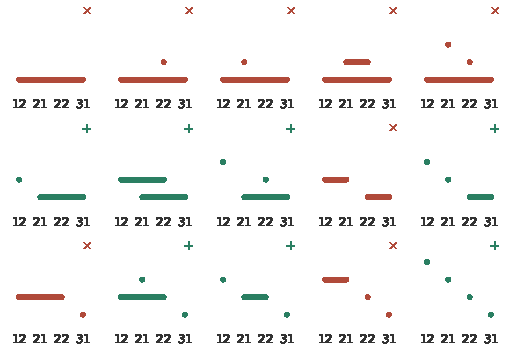
\includegraphics[width=0.98\linewidth]{figs_ws4/fig_census.pdf}
\caption{The census. Each panel draws one partition: a bar over a group
of states is a fibre (green when its common safe-action set is
nonempty, red when empty), and the margin marks adequacy
(\(+\)/\(\times\)). The two adequate two-cell partitions are panels 6
and 7 of the middle row.}
\label{fig:census}
\end{figure}

The maximal subsets with a nonempty common safe-action set are
\(\{(1,2), (2,2)\}\) and \(\{(2,1), (2,2), (3,1)\}\). They overlap in
\((2,2)\), so no partition into maximal common-action sets exists:
coarsening to maximal fibres is not an available design, and the
adequate partitions found by the census are the design options. Two
consequences follow. Pairwise intersection of safe-action sets is
necessary for fibre adequacy but not sufficient in general; and an
observation map merging states with disjoint safe-action sets obstructs
at that information state while every branch remains individually
viable --- the remedy is a fibre split, not a finer threshold on the
same index. The census makes both visible at the level of individual
fibres: in each inadequate partition of Table \ref{tab:census} the
failing fibre is exactly one merging \((1,2)\) --- whose safe-action
set is the singleton \(\{1\}\) --- with a state whose safe actions
exclude \(1\), i.e. \((2,1)\) or \((3,1)\), and each adequate
partition merges \((1,2)\) with neither.

\subsection{Regime uncertainty}\label{regimes}

Two regimes alternate: an adversary chooses at the end of step
\(t - 1\) the regime realized at step \(t\); the acting regime damages
its coordinate by two units, the other regenerates one. With frozen
regimes the kernel is \(36 = 36\): the corner \((1,1)\) is viable under
each regime separately. Mode-blind operation, with the regime read only
through the state, yields a kernel of exactly 28 --- every pair
containing the corner is lost, no merged-pair loss exists, and the loss
is generated entirely at the singleton level. The mode-blind kernel
agrees setwise with the full-information kernel of Section
\ref{classes}; the agreement is coincidental, arising under different
damage routings, and no identity is claimed.

\subsection{The continuous benchmark}\label{benchmark}

Two stocks face demand floors under one control set
\(U = \{u \ge 0 : u_1 + u_2 \ge 2\}\) with caps
\(\mathrm{cap}_1(Y) = 3/2 - (Y - 2)/10\) and
\(\mathrm{cap}_2(Y) = 59/50 - (Y - 2)/10\). The critical aggregate is
\(Y^{*} = 27/5\): the cap sum equals \(2\) exactly there. Table
\ref{tab:bench} evaluates the caps on the audited aggregates and Figure
\ref{fig:bench} displays them. The \(Y = 5\) fibre is viable with
witness \((6/5, 4/5)\); the \(Y = 6\) fibre is obstructed with cap sum
\(47/25 < 2\), certified by the dual measure \((1/2, 1/2)\) on the two
active-floor atoms with margin \(3/50\). The fibre width is
\(\Delta x_1(Y) = Y - 4\).

\begin{table}[t]
\centering
\footnotesize
\caption{The benchmark's cap arithmetic on the audited aggregates
(exact rationals). The cap sum crosses the demand level \(2\) exactly
at \(Y^{*} = 27/5\); at \(Y = 6\) the cap sum falls \(3/25\) short of
\(2\), and the normalized dual measure \((1/2, 1/2)\) certifies the
obstruction with margin \(3/50\) --- the best feasible allocation's
expected drift equals \(-3/50\).}
\label{tab:bench}
\begin{tabular}{@{}l c c c l@{}}
\toprule
\(Y\) & \(\mathrm{cap}_1\) & \(\mathrm{cap}_2\) & sum & reading\\
\midrule
4 & $13/10$ & $49/50$ & $57/25$ & above\\
$9/2$ & $5/4$ & $93/100$ & $109/50$ & above\\
5 & $6/5$ & $22/25$ & $52/25$ & viable (witness $(6/5, 4/5)$)\\
$27/5$ & $29/25$ & $21/25$ & $2$ & critical\\
$11/2$ & $23/20$ & $83/100$ & $99/50$ & below\\
6 & $11/10$ & $39/50$ & $47/25$ & obstructed, margin $3/50$\\
\bottomrule
\end{tabular}
\end{table}

\begin{figure}[t]
\centering
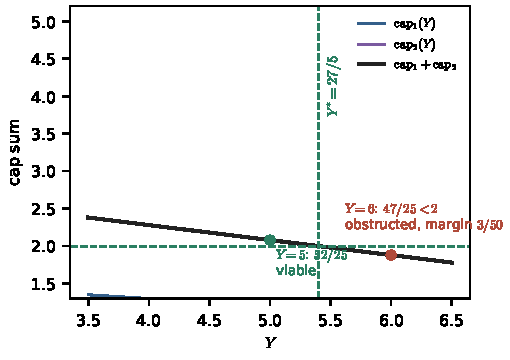
\includegraphics[width=0.96\linewidth]{figs_ws4/fig_benchmark.pdf}
\caption{The benchmark. Both caps decrease linearly in the aggregate
\(Y\); their sum crosses the demand level \(2\) exactly at
\(Y^{*} = 27/5\). The \(Y = 5\) fibre is viable (green), the \(Y = 6\)
fibre obstructed with margin \(3/50\) (red).}
\label{fig:bench}
\end{figure}

\subsection{Static duality}\label{duality}

Static duality on the two-floor instance: the max--min equals the
min-\(\lambda\) max at value \(-1/10\), with multiplier
\(\lambda = (1/2, 1/2)\) the normalized Farkas pair of the calculus's
worked certificate (Abaee, 2026b). Figure \ref{fig:duality} displays
the instance: under the normalized multiplier the expected drift is
constant \(-1/10\) on all of \([0,1]\). Convexity is load-bearing: with
\(U = \{0, 1\}\) and rows \((-1, +1)\), \((+1, -1)\), the common set is
empty, the max--min is \(-1\), and the min-multiplier maximum is
\(0\). Under convexity the witness is sparse: the Helly-tight triple
\(\{u_1 \ge 1,\ u_2 \ge 1,\ u_1 + u_2 \le 1\}\) attains the obstruction
with \(m{+}1 = 3\) points. The feasible contrast at rows
\((2/5 - u,\ u - 1/5)\) carries value \(+1/10\) on both sides of the
saddle: a certificate exists exactly where the value is nonpositive.
Weak duality holds unconditionally; strong duality holds in the
finite-horizon finite and static-observation classes.

\begin{figure}[t]
\centering
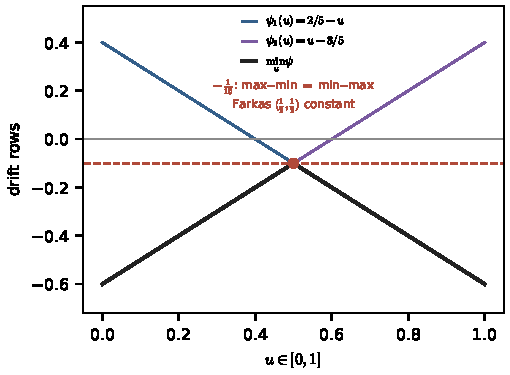
\includegraphics[width=0.96\linewidth]{figs_ws4/fig_duality.pdf}
\caption{Static duality on the two-floor instance. The two drift rows
cross at \(u = 1/2\); the max--min equals the min-multiplier maximum at
\(-1/10\), and the normalized Farkas pair \((1/2, 1/2)\) makes the
expected drift constant at the value.}
\label{fig:duality}
\end{figure}

\subsection{The certainty-equivalence drift audit}\label{drift}

For the index \(g(s) = s^{2}\) the uncorrected law's one-step drift is
\(g(s + 1/10) - g(s) = s/5 + 1/100\) on \([1,2]\): increasing, with
minimum \(21/100\) at \(s = 1\) and maximum \(41/100\) at \(s = 2\)
(Table \ref{tab:drift}); the corrected law's drift is identically zero.
A biased observation map empties a nonempty kernel under an injective
index, and the remedy is structural correction of the map, not a better
sensor.

\begin{table}[t]
\centering
\footnotesize
\caption{The certainty-equivalence drift audit:
\(g(s + 1/10) - g(s) = s/5 + 1/100\) exactly; the corrected law's
drift is \(0\) at every probed state.}
\label{tab:drift}
\begin{tabular}{@{}l c c c@{}}
\toprule
\(s\) & uncorrected & corrected & increment per \(1/4\)\\
\midrule
1 & $21/100$ & 0 & \\
$5/4$ & $26/100$ & 0 & $1/20$\\
$3/2$ & $31/100$ & 0 & $1/20$\\
$7/4$ & $36/100$ & 0 & $1/20$\\
2 & $41/100$ & 0 & $1/20$\\
\bottomrule
\end{tabular}
\end{table}

\subsection{Multiple floors}\label{floors}

With several binding floors the Farkas certificate obstructs jointly: a
single certificate over all floors certifies nonviability where
per-floor certificates do not compose. On the audited two-floor
extension, the minimal infeasible subsystem carries explicit
witnesses, and the corner \((1,1)\) is dynamically nonviable as in the
shared system. Two further objects are recorded for subsequent study: a
first-breach timing bound for multi-floor systems, and a corner-cone
reading of the infeasibility region.

\subsection{Design rules}\label{rules}

Four rules hold as identities on the audited systems and transfer as
default guidance. \emph{Timing:} reviews are boundary-inclusive ---
\(T_{\mathrm{obs}} \le \sigma^{*}(z_0)\), the deadline at worst-case
exit admissible (Section \ref{timing}). \emph{Coarseness:} a fibre
merging states with disjoint safe-action sets obstructs at that
information state; the remedy is a fibre split, not a finer threshold
on the same index (Section \ref{adequacy}). \emph{Aggregation:} an
index whose fibres cross a floor cannot support an exact
safe/unsafe verdict; the certainly-safe set is the honest report.
\emph{Bias:} the uncorrected law's drift is at least \(21/100\) on a
101-point grid of \([1,2]\), while the corrected law's drift is
identically zero; a biased observation map empties a nonempty kernel
under an injective index, and the remedy is structural correction of
the map, not a better sensor (Section \ref{drift}). To these the
decentralized audit adds a fifth: an authority restriction on one
agent's vote can collapse the sustainable set outright, so protocol
design precedes instrument tuning (Section \ref{decentralized}).

\subsection{Verification methods}\label{methods}

Every count, witness, identity, bound, figure, and tabulated entry in
this paper is regenerated by deterministic scripts in exact integer and
rational arithmetic, standard library only. The master verification
script recomputes the counts of Sections \ref{master}--\ref{regimes}
from the shared system's primitives --- the transition, the fibre
partition function, and the backward recursion with the no-repeat
protocol threaded as a parameter --- re-derives every tabulated entry of
Tables \ref{tab:master}, \ref{tab:laws}, \ref{tab:timing},
\ref{tab:census}, \ref{tab:bench}, and \ref{tab:drift} independently,
enumerates the census of Section \ref{adequacy}, evaluates the
benchmark identities of Section \ref{benchmark} in rational
arithmetic, asserts the drift bounds, and checks that each headline
number appears in the text. The figure-and-table generation script
recomputes and asserts each plotted or printed quantity from the same
primitives before drawing; the two scripts agree on every shared
quantity. The audited identities are additionally covered by the
per-system verification scripts of the companion archive (Abaee, 2026a;
see the Code availability statement).

\subsection{Conclusion}\label{conclusion}

Exact audits bind the obstruction calculus to its worked systems: each
mechanism acquires a count, a witness, and a boundary. The timing
certificate fires everywhere beyond \(z_0 - 1\) and nowhere at the
boundary; the adequate monitoring designs on the audited target are
enumerable, and no coarsest one exists; policy-class value drops
unequally across aggregation and protocol restrictions, with the two
middle cells incomparable, the meet of their kernels institutional
setwise, and exactly one pair --- the alternation-forced pair --- beyond
both; unanimity costs a fixed and identified set of beliefs, sustained
by exactly the \(4 \times 4\) product of free votes, recoverable only
while both votes remain free; regime blindness loses exactly the
corner's pairs; and the continuous benchmark separates the viable from
the obstructed at \(Y^{*} = 27/5\) with rational certificates on both
sides. The design rules --- boundary-inclusive reviews, fibre splits
over threshold tuning, certainly-safe reporting under aggregation,
structural repair of bias, and protocol design before instrument tuning
--- are the audit's operational content, and the master table is its
evidence: every count in the paper is one column of one table, every
entry of which is regenerated by script.

\subsection*{References}

Abaee, A., 2026a. Robust viability of the 2J3KL limit reference point
under a surplus-production map: policy scoring, expansion, and when
catch cannot help. Zenodo.
\url{https://doi.org/10.5281/zenodo.22552060}

Abaee, A., 2026b. An obstruction calculus for viability under
incomplete observation (submitted).

\subsection*{Declarations}

\subsection*{Funding}
None.

\subsection*{Competing interests}
None.

\subsection*{Data availability}
No external data were used.

\subsection*{Code availability}
The verification script \url{paper2_worked_systems_v4_verification.py}
and the figure-and-table generation script
\url{paper2_worked_systems_figures.py} are publicly available at
\url{https://github.com/MIKEAA2020/general-sustainability} (folder
\texttt{arena agent 1/paper rewrites/latex}); they reproduce all
counts, witnesses, bounds, figures, and tabulated entries verbatim.

\subsection*{AI declaration}
GLM (Z.ai), Qwen (Alibaba Cloud) and DeepSeek AI assisted with drafting
and iterative review. The author reviewed and edited outputs and takes
responsibility for the final work.

\end{document}
